
\section{Conception de MID}
La conception des \gls{mid} commence par la création du schéma électrique dans un logiciel de conception électronique standard, puis le schéma est exporté sous forme de \emph{netlist}, c'est à dire d'une liste de connexion entre différents composants.
Le design mécanique du \gls{mid} se fait dans un logiciel de \textsc{dao} standard, comme Solidworks, puis est exporté au format \textsc{step}.

La \emph{netlist} et le fichier \textsc{step} sont ensuite importés dans un logiciel spécifique \footnote{Nextra de chez Mecadtron \url{http://www.mecadtron.com/produkte/nextra.en.php}} pour l'étape de routage (placement des pistes).
Lors de cette étape, on place aussi des repères appelés \emph{fiducials} qui seront utilisés par les machines d'activation et d'assemblage pour faire un alignement visuel.
On peut également placer des codes-barres 2D (\emph{datamatrix}) qui seront modifiés par la machine d'activation pour y placer un numéro de série, afin d'assurer le suivi des pièces.

\subsection{Matériaux utilisables}
Les contraintes inhérentes à la technologie \gls{lds} limitent fortement le choix des matériaux :
\begin{itemize}
    \item la pièce étant injectée puis activée, le matériaux choisi doit être un thermoplastique,
    \item pour l'étape d'activation, le polymère doit pouvoir se lier avec un dopant organométallique, généralement à base de palladium,
    \item l'assemblage des composants par \textit{reflow soldering} exige une température de fusion élevée.
\end{itemize}

LPKF a donc créé une liste de matériaux utilisables et recommandés pour le \gls{lds} (voir tab. \ref{tab:mid-materials}).
Une liste de fournisseurs proposant ces matériaux déjà dopés est également disponible chez LPKF \cite{mid-design-rules}.

% Table des matériaux
\begin{table}[h]
\centering
\begin{tabular}{l l}
\toprule 
Type & Matériau \\
\midrule % In-table horizontal line
LCP & Liquid Crystal Polymer \\
PA 6/6T & Polyamide \\
PBT & Polytéréphtalate de butylène \\
PBT/PET & Mélange de PBT et de PET \\
PPA & Polyphthalamide \\
PC & Polycarbonate \\
PC/ABS & Mélange de PC et d'ABS \\ 
\bottomrule 
\end{tabular}
\caption{Matériaux utilisables comme substrat}
\label{tab:mid-materials}
\floatfoot{Source: \cite{mid-design-rules}}
\end{table}

\subsection{Limites du procédé LDS}
La conception de circuits \gls{mid} est délicate car elle doit prendre en compte des limites provenant de l'injection plastique, de l'activation laser et de la métallisation.
L'ingénieur doit donc porter un soin tout particulier à la conception, car de petits détails, comme des trous borgnes, peuvent augmenter significativement le coût de la pièce, voir même la rendre impossible à réaliser.
L'ensemble des règles de conception à respecter est compilée dans un seul document, fourni par LPKF \cite{mid-design-rules}.
Nous allons ici nous concentrer sur les plus importantes.

La plus grosse limitation des \glspl{mid} par rapport aux \glspl{pcb} est la faible densité de pistes atteignable.
En effet, il est impossible de fabriquer des \glspl{mid} avec des couches internes, là où des circuits à 16 couches sont facilement atteignables dans le domaine des \glspl{pcb}.
De plus, les \glspl{mid} ne permettent pas de faire des pistes très fines ou très serrées : on considére généralement qu'il faut rester au-dessus de \SI{150}{\micro\meter} pour la largeur de piste et \SI{200}{\micro\meter} pour l'écart inter-piste.

De plus, l'angle d'incidence du laser (correspond à l'angle $\beta$ sur la fig. \ref{fig:angle-limit}) doit rester inférieur à \SI{30}{\degree} par rapport à la normale de la surface.
Un angle plus important change la forme du spot du laser, qui passe d'un cercle à une ellipse, ce qui dissipe trop la puissance du laser et diminue la résolution.
On peut néanmoins corriger ce problème en montant la pièce sur un support orientable, moyennant une perte de temps pour la rotation de la pièce et le réalignement optique de la machine.
Un autre moyen de corriger ce problème est d'utiliser une machine avec plusieurs lasers orienté indépendamment.
Dans les cas les plus extrêmes, on ne peut pas corriger ce problème de cette façon, et alors le passage au two-shot est inévitable.
On préfère cependant souvent modifier la pièce pour rester sur une technologie \gls{lds} pour minimiser les coûts et faciliter le développement.

\begin{figure}[h]
    \begin{center}
        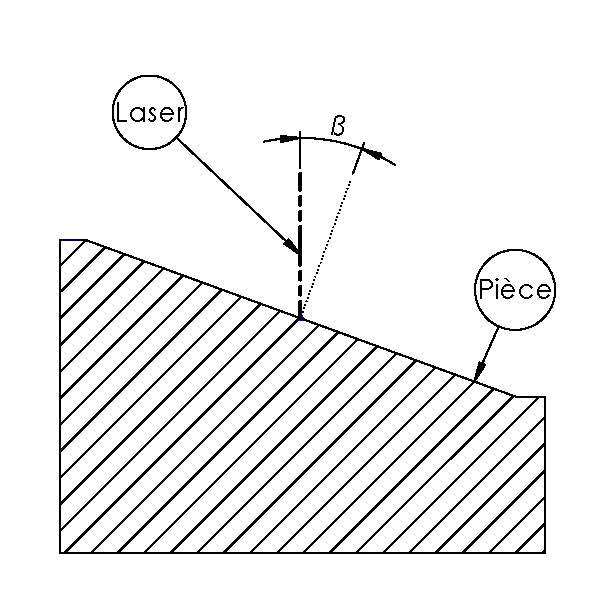
\includegraphics[width=0.5\textwidth]{images/activation_limit}
        \caption{Angle limite pour l'activation ($\beta < \SI{30}{\degree}$).}
        \label{fig:angle-limit}
    \end{center}
\end{figure}

La dernière limitation concerne le volume de travail de la machine d'activation laser : environ $\SI{200}{\milli\meter}\times\SI{200}{\milli\meter}\times\SI{25}{\milli\meter}$, légèrement variable d'une machine à l'autre.

\subsection{Prototypage}
Le travail d'ingénieur étant un procédé itératif, il est important de pouvoir réaliser rapidement et à faible coût des prototypes fonctionnels d'une pièce ou d'un système.
Le \gls{mid}, et plus particuliérement l'étape d'injection plastique, n'est pas bien adapté au prototypage : lancer une série coûte cher et n'est pas un procédé rapide (jusqu'à six semaines).

Le \gls{lds} offre cependant différentes possibilités de prototypage simples, puisque la seule étape différente de la production est la création de la pièce de base en polymère.
Les étapes d'activation et de métallisation sont donc inchangées par rapport à la production.
Le prototypage sert autant à mettre au point le \gls{mid} que le procédé de production, par exemple les supports pour la métallisation ou l'activation.

La première méthode (et la plus simple) pour prototyper une pièce en \gls{mid} consiste à usiner sa forme dans un bloc de polymère déjà dopé.
On utilise donc des machines d'usinage conventionelles ou \textsc{cnc}, qui sont facilement disponibles, avant d'activer et de métalliser la pièce.
Cette méthode a comme avantage de ne demander aucun équipement spécifique et d'être facilement réalisable par un opérateur sans formation sur une machine spéciale.
Son principal inconvénient est que certaines pièces qui peuvent être injectées ne peuvent pas être usinées et inversement, ce qui rend cette technique inutile pour certaines pièces.

Une seconde méthode de prototypage consiste à réaliser en stéréolithographie ou en impression 3D la forme de la pièce puis à la peindre avec une laque spéciale vendue par LPKF, qui rend la surface activable après un bref passage au four, ce qui demande un polymère stable à \SI{90}{\celsius}.
On utilisera donc de préférence de l'\textsc{abs}.
Cette méthode, comme la précédente, permet de réduire à environ une semaine le temps entre l'envoi d'une commande et la réception d'un prototype.

Toujours en utilisant la stéréolithographie ou l'impression 3D, il est possible de réaliser la forme de la pièce en positif, puis de couler un moule en silicone autour, pour l'utilisation dans une machine d'injection sous vide.
On injecte ensuite la pièce en \textsc{pur} dopé, qu'on peut activer et métalliser de façon standard.
Cette méthode a comme principal inconvénient de demander une machine spécifique pour l'injection sous vide, et ne de pas proposer de grands avantages par rapport aux deux méthodes précédentes.
Elle n'est donc que rarement utilisée.

La dernière méthode de prototypage est résérvée aux derniers tests avant la production en grande série, car c'est la plus onéreuse.
Dans cette méthode, tout le procédé est rigoureusement identique au procédé final, la seule différence étant le type de moule : on utilise ici un \textit{soft mold} en aluminium, plutôt qu'un moule en acier trempé.
On arrive donc à un moule se comportant comme le vrai, ce qui est important pour tester tous les paramètres d'injection (température, vitesse d'injection, etc.), à un prix bien moindre : un \textit{soft mold} coûte environ 10\% du prix de son homologue en acier, mais ne permet de produire que 1000 pièces environ.
\subsection{Comparatif entre PCB et MID}
Il est important de noter que les \glspl{mid} ne sont pas un remplaçant ou un successeur aux \glspl{pcb} : ils répondent à des besoins différents.
Par exemple, réaliser un circuit complexe mais sans intégration mécanique, comme une carte mère d'ordinateur, en \gls{mid} n'est pas une bonne idée : la densité de pistes et d'éléments est beaucoup plus grande avec un \gls{pcb}, tandis que les seules fonctions mécaniques demandées sont des perçages de fixations au boîtier.
En revanche, dans le cas d'un ordinateur portable, la réalisation d'une antenne \gls{mid} (WiFi, Bluetooth, etc.) est intéressante, étant donné son intégration facilitée au châssis.
On voit dans cet exemple que la combinaison d'un \gls{mid} et d'un \gls{pcb} permet de tirer le meilleur des deux technologies.

En résumé, les principaux avantages des \glspl{mid} sont :
\begin{itemize}
    \item les \glspl{mid} permettent une géométrie en trois dimensions tandis que les \glspl{pcb} sont limités à un plan,
    \item ils permettent d'associer des fonctions mécaniques et électriques dans une seule pièce,
    \item la complexité (et donc le temps d'assemblage) est réduit par les \glspl{mid}, grâce à la diminution du câblage.
\end{itemize}

~

A l'inverse, leurs principaux inconvénients sont :
\begin{itemize}
    \item les circuits en \gls{mid} ne permettent pas une grande densité de pistes, car il n'est pas possible de faire des couches internes et que la résolution du procédé est limitée,
    \item l'assemblage des composants est plus difficile, car pas limité à un seul plan,
    \item faire des petites séries de \gls{mid} est possible, mais très cher, tandis que les \glspl{pcb} sont plus abordables car ils ne demandent pas de moules.
\end{itemize}
